\documentclass[12pt]{article}

% -- Packages

\usepackage{amsmath}
\usepackage{amsthm}
\usepackage{amssymb}
\usepackage{graphicx}
\usepackage{float}
\usepackage{multirow}
\usepackage{xcolor}
\usepackage{algorithmic}
\usepackage[ruled,vlined,commentsnumbered,titlenotnumbered]{algorithm2e}
\usepackage{array}
\usepackage{booktabs}
\usepackage{url}
\usepackage{parskip}
\usepackage[margin=1in]{geometry}
\usepackage[T1]{fontenc}
\usepackage{cmbright}
\usepackage[many]{tcolorbox}
\usepackage{enumitem}
\usepackage{hyperref}
\usepackage[font=small,labelfont=bf]{caption}
\documentclass{article}
\usepackage[table,xcdraw]{xcolor}
% -- Macros

\newcommand{\HWNum}{5}
\newcommand{\Rule}{\rule{\linewidth}{0.5pt}}
\newcommand{\Expecting}[1]{[\textbf{We are expecting:} #1]}
\newcommand{\Points}[1]{\textbf{(#1 pt.)}}




\begin{document}
 \begin{center}
	    \section*{ARM Limited} 
	    \section*{CS262-Design Document} \hfill
	    \begin{figure}[!ht]
	            \begin{center}
	                
\includegraphics[width=50mm]{logo.png}
	            \end{center}
        \end{figure}  
        \begin{center}
        \section*{Project Supervisor}
            \subsection*{Mr. Samyan Qayyum Wahla}
            \subsection* {}
            \subsection* {}
        \end{center}
        \begin{center}
	    \section*{Project Members(G-5) }
	        \subsection*{Mukarram Ali       2021-CS-58}
	        \subsection*{Rayan Rasheed      2021-CS-59}
	        \subsection*{Ammad Aslam        2021-CS-67} \hfill
	     \hfill \break 
      \end{center}
	    \section*{DEPARTMENT OF COMPUTER SCIENCE}
	    \subsection*{UNIVERSITY OF ENGINEERING AND TECHNOLOGY, Lahore}
	    \subsection*{Pakistan}
     
	    \newpage
	\end{center}


	\Rule
\tableofcontents
\section{Project Description}
We are facing not just a challenging business environment but a rapidly changing one. There is always room for improvement. Running a Distribution System without a proper application can lead to many problems. In the warehouse, by not managing your stock count, cost price changes and not being able to view your stock position can have drastic consequences. The company has no way of knowing how much stock is left in your warehouses and how much you’ve sold out. If you don’t know how much you have left, you can’t restock your inventory which will cause delays and frustrate your customers. It is important to track your inventory so that you can plan ahead effectively. The company is unable to keep a record of its employees, day-to-day sales and profits, customer information and transportation cost. Searching a 10-year-old record for the company is extremely challenging. Speed is also critical when ensuring that you get the correct items picked, packed and distributed to the correct address and client. Understanding the right approach to solving these challenges is essential for distributors to adapt, transform and differentiate themselves in this new challenging business landscape.  \\
We are all aware that we live in an increasing electronic world. Simply put if the Distribution Company is not using a proper, well-managed application then it is facing commercial suicide. So, our Project aims to develop such an application for the Company that can address all the above problems and help the company improve the distribution system and management of the company processes. \\
The administrator of the application is the General Manager of the company. He can hire the company employees (sales agent), riders (to deliver the packages) and an inventory Manager. He is in the charge of each module. Each employee would have their individual accounts. The inventory Manager is in charge of the warehouse, keeping the record of the product as being delivered by the Manufacturing Company. The sales agent will deal with the clients, their orders and assign the delivery task to the riders depending upon the location assigned to them. The rider would be a given a specific area in which he would have to deliver all the goods and complete all its orders in the given time. Further bonuses will be given according to the statistic chart at the end of the month. \\
The Distribution Company that we have plumped for is the Shoe Distribution Company. A well-recognized shoe Manufacturing Company ADIDAS is our manufacturer. The implementation of this application will work with a company called ARM. As a distribution company we deliver the products to numerous retailers, wholesalers, concept stores, buyers and agents all over the Lahore. It operates on its own as it is an independent company establishing a connection between the products and the client. \\
The Record and performance are also evaluated automatically in order to provide the appraisal. The company established the excellent track record for the best customer satisfaction. As a footwear sourcing company, we also provide sustainable material sourcing options to help our clients choose a greener path. An organization’s main focus must be to satisfy its customers and in order to do so we are providing a refund policy for the client and email verification after the order had been sent to them. Sometimes, the rider doesn’t deliver the parcel to the exact location. So, to overcome this problem we provide the rider with the exact location of client on Google map. The client should place the minimum required order then the sales agent would request the inventory manager for the confirmation of the stock. The application also maintains the daily attendance of the employees, the scheduling of the riders and fuel consumption cost. The clients would also be informed of the special offers. Our system is cited as the most efficient tool that is at the company’s disposal. \\
The application offers three modes. \\
•	Manager authorized mode. \\
•	Sales Agent authorized mode. \\
•	Inventory Supervisor mode \\
•	Rider authorized mode. \\
	

\section{Project Features:}
•	User interface screen will be operated according to the role of the person who signs in. \\
•	Client can pay in installments or pay in advance. \\
•	Rider will be informed with the stock availability during placing orders. If the required order of the client is out of stock, order could not be placed and an email would be sent to the Inventory Supervisor to inform about stock unavailability. \\
•	Sales Agent will assign the location of decided area to the Rider. The order will be delivered the very next day. \\
•	Rider could only deliver limited number of orders in a single day. \\
•	Attendance of all employees. \\

\section{Technology Stack}
\begin{table}[H]
\begin{tabular}{|l|l|}
\hline
Language & 1. Python                 \\ \hline
IDEs     & 1.Visual Studio Community \\
         & Visual Studio Code        \\ \hline
\end{tabular}
\end{table}

\section{Project actors}
\begin{table}[H]
\begin{tabular}{|l|l|}
\hline
Actor Name  & Manager                                                                                                                                                                                                                                                                                                                    \\ \hline
Actor Type  & Primary                                                                                                                                                                                                                                                                                                                    \\ \hline
Description & \begin{tabular}[c]{@{}l@{}}Manager can hire and fire employees to the Company. He can   view all the records\\  or monthly reports and stock. He also has to check the   performances at all times, \\ check inventory. He gives monthly incentives to   all the employees according to \\ their performance.\end{tabular} \\ \hline
\end{tabular}
\end{table}

\begin{table}[H]
\begin{tabular}{|l|l|}
\hline
Actor Name  & Inventory   Supervisor                                                                                                                                                                                                                                                                                                                                                                                   \\ \hline
Actor Type  & Primary                                                                                                                                                                                                                                                                                                                                                                                                  \\ \hline
Description & \begin{tabular}[c]{@{}l@{}}This system will also have an inventory   supervisor. He will manage inventory\\  in the warehouse and will notify the   general manager whenever a new order\\  should be made. He can buy stock from   the supplier after the approval of the\\  General Manager. He will provide   authorization to the rider after checking\\  the stock from the warehouse.\end{tabular} \\ \hline
\end{tabular}
\end{table}

\begin{table}[H]
\begin{tabular}{|l|l|}
\hline
Actor Name  & Sales Agent                                                                                                                                                                                                                                                                                                                                                  \\ \hline
Actor Type  & Primary                                                                                                                                                                                                                                                                                                                                                      \\ \hline
Description & \begin{tabular}[c]{@{}l@{}}Sales Agent will also have an account of its own. He will   keep a track of all the \\ orders of the riders and their information. He will   assign a specific area to a \\ specific rider. He can also update the location   of riders. He will sendout email to\\  the client after the delivery of the   product.\end{tabular} \\ \hline
\end{tabular}
\end{table}

\begin{table}[H]
\begin{tabular}{|l|l|}
\hline
Actor Name  & Rider                                                                                                                                                                                                                                                                                                                                                                                                                                                                       \\ \hline
Actor Type  & Primary                                                                                                                                                                                                                                                                                                                                                                                                                                                                     \\ \hline
Description & \begin{tabular}[c]{@{}l@{}}The Rider has most of the responsibilities in the system.   Rider will take order \\ from the shopkeepers and deliver the order afterwards.   Rider   is able to see the\\  products when creating an order. He can view the history of his   delivered orders \\ and can also view pending orders (to be delivered). He will   send out email to \\ sale agent about the order placement. He can add and update   the client data.\end{tabular} \\ \hline
\end{tabular}
\end{table}

\begin{table}[H]
\begin{tabular}{|l|l|}
\hline
Actor Name  & FBR                                                                                                                                                                                                                                   \\ \hline
Actor Type  & Off-Stage Actor                                                                                                                                                                                                                       \\ \hline
Description & \begin{tabular}[c]{@{}l@{}}FBR collect tax from companies from their earned profits   under the tax \\ ordinance law, 2001. It is pertinent for all registered   companies to pay tax to \\ work legally across country.\end{tabular} \\ \hline
\end{tabular}
\end{table}



\section{Use Cases}
\subsection{Reset Password:}

\begin{table}[H]
\begin{tabular}{|l|l|}
\hline
Use Case ID & U01                                                                        \\ \hline
Name        & Reset Password                                                             \\ \hline
Actor       & The Manager, Rider, Inventory Supervisor and Sales agent.                  \\ \hline
Description & If the user forgets his/her password, they can reset it.                   \\ \hline
Flow        & Base Flow:                                                                 \\
            & 1.The user opens the application.                                          \\
            & 2.He enters the email and password.                                        \\
            & 3.He clicks on login.                                                      \\
            & 4.A message box appears containing the message “Not matched in Data Base”. \\
            & 5.He clicks on forget password.                                            \\
            & 6.After clicking, he receives an email containing the new password.        \\
            & Repeats step 1-3                                                           \\
            & 7.Successfully login in the main page.                                     \\ \hline
\end{tabular}
\end{table}

\subsection{Add Employee}

\begin{table}[H]
\begin{tabular}{|l|l|}
\hline
Use Case ID & U02                                                                                                                                                                                                                                                                                                                                                                                                                                                                                                                                                                                                                                                                            \\ \hline
Name        & Add Employee                                                                                                                                                                                                                                                                                                                                                                                                                                                                                                                                                                                                                                                                   \\ \hline
Actor       & The Manager                                                                                                                                                                                                                                                                                                                                                                                                                                                                                                                                                                                                                                                                    \\ \hline
Description & \begin{tabular}[c]{@{}l@{}}The Manager can add a new   employee to the company. It could either be the\\  rider, sales agent, workers   or the inventory supervisor. He would take the \\ name, email, CNIC, address,   phone number, bank account of the employee.\\  After filling out the details, he   will give them a password and status and a \\ base salary depending upon the   status.\end{tabular}                                                                                                                                                                                                                                                                 \\ \hline
Flow        & \begin{tabular}[c]{@{}l@{}}Base Flow:   \\ 1.Customer   arrives at company.  \\ 2.Fill out   the form to give interview. \\ 3.After   passing interview, he will officially become company’s employee.\\  To give him   access to the application, the manager will register that \\ employ by entering all his details which include his name, CNIC, E-mail\\  address, status, bank   account, telephone number.\\ 4.After   entering all his information, he has given his login details to\\  login into application.\\ Alternative Flow:\\                  3a.The employee is a rider.\\                        1.He also assigns a   vehicle to the rider.\end{tabular} \\ \hline
\end{tabular}
\end{table}

\subsection{Deduction of Fuel Money:}

\begin{table}[H]
\begin{tabular}{|l|l|}
\hline
Use Case ID & U03                                                                                                                                                                                                                                                                                                                                                  \\ \hline
Name        & Deduction of Fuel Money                                                                                                                                                                                                                                                                                                                              \\ \hline
Actor       & The Manager                                                                                                                                                                                                                                                                                                                                          \\ \hline
Description & \begin{tabular}[c]{@{}l@{}}The rider will send a report to the Manager on a weekly   or daily basis about the\\  fuel consumption depending. Depending upon that   report money will be \\ deducted from the company account automatically by the   confirmation of the\\ Manager.\end{tabular}                                                      \\ \hline
Flow        & \begin{tabular}[c]{@{}l@{}}Base Flow:  \\ 1.The rider   opens the fuel report. \\ 2.Adds all the   information about fuel consumption.\\ 3.After   clicking sent report, the Manager will receive the report. \\ 4.The Manager   will open finance module and will delete the total amount of \\ money spend on   fuel of each vehicle.\end{tabular} \\ \hline
\end{tabular}
\end{table}


\subsection{Give Salaries:}

\begin{table}[H]
\begin{tabular}{|l|l|}
\hline
Use Case ID & U04                                                                                                                                                                                                                                                                                                                                                                                                                                                                                                                                                                                                                                                                                                                                                                                                                                                                                                                                                              \\ \hline
Name        & Give Salaries                                                                                                                                                                                                                                                                                                                                                                                                                                                                                                                                                                                                                                                                                                                                                                                                                                                                                                                                                    \\ \hline
Actor       & The Manager                                                                                                                                                                                                                                                                                                                                                                                                                                                                                                                                                                                                                                                                                                                                                                                                                                                                                                                                                      \\ \hline
Description & The Manager is in the charge   of giving salaries to all the employees.                                                                                                                                                                                                                                                                                                                                                                                                                                                                                                                                                                                                                                                                                                                                                                                                                                                                                          \\ \hline
Flow        & \begin{tabular}[c]{@{}l@{}}Base Flow:   \\ 1.The Manager logged into the   system. \\ 2.He clicks   on the Finance button and from the dropdown menu, he selects \\ “Salaries”.\\ 3.Now he can   view the all the employees and the salary that is needed to be\\  paid to them.\\ 4.When the   manager clicks pay button, money will be transferred to their \\ account and   deducted from the company account.\\ 5.A message   box will be shown of successfully transaction of money.\\ 6.An email   would be sent out to the employee being paid.\\ Alternative flow:\\             1a.The Manager forgets his password.\\                    1.He clicks   on ‘Forgot Password’ to recover his account.\\             4a.Company account does not have   enough money to pay the employees.\\                    1.He will   debit into the company account.  \\                    2.He requests   the employee to get paid in installments.\end{tabular} \\ \hline
\end{tabular}
\end{table}

\subsection{Give Bonuses}

\begin{table}[H]
\begin{tabular}{|l|l|}
\hline
Use Case ID & U05                                                                                                                                                                                                                                                                                                                                                                                                                                                                                                                                                                                                                                                                                                                                                                                                                           \\ \hline
Name        & Give Bonus                                                                                                                                                                                                                                                                                                                                                                                                                                                                                                                                                                                                                                                                                                                                                                                                                    \\ \hline
Actor       & The Manager                                                                                                                                                                                                                                                                                                                                                                                                                                                                                                                                                                                                                                                                                                                                                                                                                   \\ \hline
Description & \begin{tabular}[c]{@{}l@{}}The Manager give bonuses to riders and sales agent   depending upon their \\ monthly performances based upon bar chart.\end{tabular}                                                                                                                                                                                                                                                                                                                                                                                                                                                                                                                                                                                                                                                               \\ \hline
Flow        & \begin{tabular}[c]{@{}l@{}}Base Flow:   \\ 1.The Manager   logged into the system.\\ 2.He clicks   on the Finance button and from the dropdown menu, he selects \\ “Salaries”. \\ 3.Two bar   graphs will be shown to him. First will be of the rider performances\\  based on   their total orders and sales agent depending upon the working days. \\ 4.He will select   the employee and click on Bonus button.\\ 5.A pop up   will be shown in which he will input the bonus amount ranging \\ from 10   thousand to 20 for rider and 5 to 10 thousand for the sales agent.\\ 6.He clicks   on pay and the money will be transferred to the employee.\\ Alternative flow:\\             1a.The Manager forgets his password.\\                    1.He clicks   on ‘Forgot Password’ to recover his account.\end{tabular} \\ \hline
\end{tabular}
\end{table}

\subsection{Update Employee:}

\begin{table}[H]
\begin{tabular}{|l|l|}
\hline
Use Case ID & U06                                                                                                                                                                                                                                                                                                                                                                                                                                                                                                                                                                                                                                                                                                                \\ \hline
Name        & Update Employee                                                                                                                                                                                                                                                                                                                                                                                                                                                                                                                                                                                                                                                                                                    \\ \hline
Actor       & The Manager                                                                                                                                                                                                                                                                                                                                                                                                                                                                                                                                                                                                                                                                                                        \\ \hline
Description & \begin{tabular}[c]{@{}l@{}}The Manager is able to update   employees by clicking the button that list the \\ employees and then select the   employee whose information needs to be update.\end{tabular}                                                                                                                                                                                                                                                                                                                                                                                                                                                                                                           \\ \hline
Flow        & \begin{tabular}[c]{@{}l@{}}Base Flow: \\ \\ 1.The Manager   logged into the system.\\ 2.An employee   comes to him and asks to change some information about him.\\ 3.The Manager   clicks on the button and gets the list of all the employees of the \\ company.\\ 4.He searches   for that particular employee.\\ 5.He clicks   and updates the information that is required to be updated.\\ Alternative Flow:\\                   1a. The Manager forgets his   password.\\                         1. He clicks on   ‘Forgot Password’ to recover his account\\                   4a. The   employee name does not found in the data base.\\                         1. The   Manager uses U02.\end{tabular} \\ \hline
\end{tabular}
\end{table}

\subsection{Add Vehicle:}

\begin{table}[H]
\begin{tabular}{|l|l|}
\hline
Use Case ID & U07                                                                                                                                                                                                                                                                                                                                                                                                                                                                                                                                              \\ \hline
Name        & Add Vehicle                                                                                                                                                                                                                                                                                                                                                                                                                                                                                                                                      \\ \hline
Actor       & The Manager                                                                                                                                                                                                                                                                                                                                                                                                                                                                                                                                      \\ \hline
Description & The Manager is able add buy a new vehicle for the riders to deliver the products.                                                                                                                                                                                                                                                                                                                                                                                                                                                                \\ \hline
Flow        & \begin{tabular}[c]{@{}l@{}}Base Flow:   \\ 1.The Manager   logged into the system.\\ 2.Today is   the day to buy a new vehicle.\\ 3.He clicks   on the button of add vehicle.\\ 4.Enters the   truck model number and fuel average of that truck.\\ 5.Enters the   price of that vehicle.\\ 6.Clicks add.\\ 7.Money gets   deducted from the company account.\\ Alternative Flow:\\                   1a. The Manager forgets his   password.\\                         1. He clicks on   ‘Forgot Password’ to recover his account.\end{tabular} \\ \hline
\end{tabular}
\end{table}


\subsection{Delete Employee:}

\begin{table}[H]
\begin{tabular}{|l|l|}
\hline
Use Case ID & U08                                                                                                                                                                                                                                                                                                                                                                                                                                                                                                                                                                                                                                                                \\ \hline
Name        & Delete Employee                                                                                                                                                                                                                                                                                                                                                                                                                                                                                                                                                                                                                                                    \\ \hline
Actor       & The Manager                                                                                                                                                                                                                                                                                                                                                                                                                                                                                                                                                                                                                                                        \\ \hline
Description & \begin{tabular}[c]{@{}l@{}}The Manager gets to fire the   employee by deleting his information from the \\ Database or when any employee   leaves the company.\end{tabular}                                                                                                                                                                                                                                                                                                                                                                                                                                                                                        \\ \hline
Flow        & \begin{tabular}[c]{@{}l@{}}Base Flow: \\ 1.The Manager   logged into the system.\\ 2.An employee   comes to him and asks to resign\\ 3.The Manager   clicks on delete employee option.\\ 4.The Manager   gets the list of all the employees of the company.\\ 5.He searches   for that particular employee.\\ 6.He clicks   and deletes that employee.\\ Alternative Flow:\\                   1a. The Manager forgets his   password.\\                         1. He clicks on   ‘Forgot Password’ to recover his account\\ 5a. The   employee is a rider.\\       1. The vehicle associated with is now   free and can be assign to any new rider.\end{tabular} \\ \hline
\end{tabular}
\end{table}

\subsection{Buy Stock:}

\begin{table}[H]
\begin{tabular}{|l|l|}
\hline
Use Case ID & U09                                                                                                                                                                                                                                                                                                                                                                                                                                                                                                                                                                                                                                                                                                                                                                                                                                                                                                                                                                                                                                                                                                                                                                                                          \\ \hline
Name        & Buy Stock                                                                                                                                                                                                                                                                                                                                                                                                                                                                                                                                                                                                                                                                                                                                                                                                                                                                                                                                                                                                                                                                                                                                                                                                    \\ \hline
Actor       & Inventory Supervisor                                                                                                                                                                                                                                                                                                                                                                                                                                                                                                                                                                                                                                                                                                                                                                                                                                                                                                                                                                                                                                                                                                                                                                                         \\ \hline
Description & \begin{tabular}[c]{@{}l@{}}Inventory Supervisor will be   able to buy the products according to its \\ requirement. Before placing the   order, he will get confirmation from the manager\\  through the email and we are   assuming the products will be reached after one \\ day and check-in by inventory   manager. Moreover, manager can also buy stock.\end{tabular}                                                                                                                                                                                                                                                                                                                                                                                                                                                                                                                                                                                                                                                                                                                                                                                                                                   \\ \hline
Flow        & \begin{tabular}[c]{@{}l@{}}Base Flow:\\ 1.Supervisor   will click the Buy stock button in the side bar menu.\\ 2.Buy Stock   page will be shown to the supervisor.\\ 3.He can see   how much products are available in the stock.\\ 4.He can   place the order by filling the information like product name, size, \\ quantity,   category, color, and then clicking on the Buy Product button.\\ 5.After this,   price of individual product and the price of total placed order will \\ be shown   to him.\\ 6.Here the   constraint will be applied that he cannot place the order when he buys\\    product less than a certain quantity.\\ 7.The manager   will receive the confirmation email from the supervisor. It is upon\\  him   whether he confirms the order or he cancels the order. \\ 8.When he   receives the confirmation email from the manager then the confirmed\\  order   will be placed.\\ 9.The order   will be added in the stock after one day.\\ Alternative Flow:\\      8a. In case supervisor receives the   rejection email from the manager then he \\ cannot place order.                \\             1. The inventory Supervisor will   cancel the order.\end{tabular} \\ \hline
\end{tabular}
\end{table}

\subsection{Update Stock:}

\begin{table}[H]
\begin{tabular}{|l|l|}
\hline
Use Case ID & U10                                                                                                                                                                                                                                                                                                                                                                                                                                                                                                                                                                                                                                                                                                                                                                                                                                                           \\ \hline
Name        & Update Stock                                                                                                                                                                                                                                                                                                                                                                                                                                                                                                                                                                                                                                                                                                                                                                                                                                                  \\ \hline
Actor       & Inventory Supervisor                                                                                                                                                                                                                                                                                                                                                                                                                                                                                                                                                                                                                                                                                                                                                                                                                                          \\ \hline
Description & \begin{tabular}[c]{@{}l@{}}Inventory supervisor will be   able to update the stock when the order will be \\ delivered by the rider. He   can also view the pending orders and the completed \\ orders.\end{tabular}                                                                                                                                                                                                                                                                                                                                                                                                                                                                                                                                                                                                                                          \\ \hline
Flow        & \begin{tabular}[c]{@{}l@{}}Base Flow: \\ 1.Supervisor   when click on the Update stock button, Update stock screen will \\ be shown to   him that contains a table with each row containing the placed and\\  confirmed   orders.\\ 2.He can   update the stock by clicking on the checkout button when the order \\ will be   delivered successfully and automatically these things will be deducted \\ from   the warehouse stock.\\ 3.When   supplier deliver its order to the warehouse, then supervisor clicks on the\\    checkout button and the stock will be added in the warehouse.\\ Alternative Flow:\\                   2a. The order has not been   delivered yet and the supervisor clicks the \\     checkout button then message box will be shown to him that contains   the \\ message that you cannot update the stock now.\end{tabular} \\ \hline
\end{tabular}
\end{table}

\subsection{Inventory Report:}

\begin{table}[H]
\begin{tabular}{|l|l|}
\hline
Use Case ID & U11                                                                                                                                                                                                                                                                                                                                                                                                                                                                                                                                                                                                                                                                                                                                                                                                                                                                                      \\ \hline
Name        & Inventory Report                                                                                                                                                                                                                                                                                                                                                                                                                                                                                                                                                                                                                                                                                                                                                                                                                                                                         \\ \hline
Actor       & Inventory Supervisor                                                                                                                                                                                                                                                                                                                                                                                                                                                                                                                                                                                                                                                                                                                                                                                                                                                                     \\ \hline
Description & \begin{tabular}[c]{@{}l@{}}Inventory supervisor will be   able to view a table containing the products of all\\  categories and their   quantity in the stock. He can also check the history of the\\  placed orders   from the suppliers with their bills.\end{tabular}                                                                                                                                                                                                                                                                                                                                                                                                                                                                                                                                                                                                                 \\ \hline
Flow        & \begin{tabular}[c]{@{}l@{}}Base Flow:\\ 1.Supervisor   when click on the Inventory Report button, dropdown will be \\ shown to him that   contains two buttons.\\ 2.First   button would be View Stock, when he clicks this button, he will be able to\\  view the products of all the categories with their available quantity in the   stock.\\  He can check the performance of each product with respect to their   sales record\\  history by clicking the Check Performance button. By clicking   this button, the\\  performance graph will be shown to him. \\ 3.Second   button would be View History, when he clicks this button, he will \\ be able to   view the history of the changes in the stock i.e. when the new order\\  was   placed and added in the stock or when the products were taken from the\\  stock   to be delivered to the customer/client.\end{tabular} \\ \hline
\end{tabular}
\end{table}

\subsection{Report Cost}

\begin{table}[H]
\begin{tabular}{|l|l|}
\hline
Use Case ID & U12                                                                                                                                                                                                                                                                                                                                                                                                                                                                                                          \\ \hline
Name        & Report Cost                                                                                                                                                                                                                                                                                                                                                                                                                                                                                                  \\ \hline
Actor       & Inventory Supervisor                                                                                                                                                                                                                                                                                                                                                                                                                                                                                         \\ \hline
Description & \begin{tabular}[c]{@{}l@{}}Inventory supervisor can   report holding, carrying and total costs. He will calculate \\ the selling cost   of the product after calculating all the company expenses.\end{tabular}                                                                                                                                                                                                                                                                                              \\ \hline
Flow        & \begin{tabular}[c]{@{}l@{}}Base Flow:  \\ 1.Supervisor   when click on the Report Cost button, the UI screen containing the \\ inputs   will be shown.\\ 2.He will   fill out all the inputs like Product buying cost, Company expenses,   \\ Government Tax, Profit percentage, etc. and then click on the calculate   button.\\ 3.After   clicking the calculate button the selling price of this product will be shown \\   and that product will be delivered to the customer at that price\end{tabular} \\ \hline
\end{tabular}
\end{table}

\subsection{Take Order:}

\begin{table}[H]
\begin{tabular}{|l|l|}
\hline
Use Case ID & U13                                                                                                                                                                                                                                                                                                                                                                                                                                                                                                                                                                                                                                                                                                                                                                                                                                                                                                                                                                                                                                                                               \\ \hline
Name        & Take Order                                                                                                                                                                                                                                                                                                                                                                                                                                                                                                                                                                                                                                                                                                                                                                                                                                                                                                                                                                                                                                                                        \\ \hline
Actor       & Rider                                                                                                                                                                                                                                                                                                                                                                                                                                                                                                                                                                                                                                                                                                                                                                                                                                                                                                                                                                                                                                                                             \\ \hline
Description & \begin{tabular}[c]{@{}l@{}}Rider will reach his assigned   location and take order from the Shop Keeper. The \\ information taken by the   rider will reach to the sales agent and then sales agent \\ will perform its   certain actions.\end{tabular}                                                                                                                                                                                                                                                                                                                                                                                                                                                                                                                                                                                                                                                                                                                                                                                                                           \\ \hline
Flow        & \begin{tabular}[c]{@{}l@{}}Base Flow:  \\ 1.Rider   reaches the Shop Keeper and he presses the Take Order button.\\ 2.Take Order   screen will open where he can see all the products available with their\\    prices and then he takes the order details like Product category, name and   quantity.\\ 3.After   taking the details from shop keeper he presses the place order button. In   \\ result of it the information will be delivered to the sales agent.\\ 4.The receipt   will be generated on which the total payment will be shown.\\ 5.Customer   can pay in advance, cash on delivery or in installments.\\ 6.Constraint   will be applied on the rider that he cannot take orders more than the   \\ assigned numbers to him.\\ Alternative Flow:\\                   5a. There are two   possibilities\\       1. If the shopkeeper places the order   first time then he has to pay the payment \\ in advance.\\       2. If he is already an existing   customer then he has the option to pay the \\ payment on delivery or in   installments.\end{tabular} \\ \hline
\end{tabular}
\end{table}

\subsection{Add Client:}

\begin{table}[H]
\begin{tabular}{|l|l|}
\hline
Use Case ID & U14                                                                                                                                                                                                                                                                                                                                                                                                                                                                                                                                                                                                                                                                                                                                                                                                                                  \\ \hline
Name        & Add Client                                                                                                                                                                                                                                                                                                                                                                                                                                                                                                                                                                                                                                                                                                                                                                                                                           \\ \hline
Actor       & Rider                                                                                                                                                                                                                                                                                                                                                                                                                                                                                                                                                                                                                                                                                                                                                                                                                                \\ \hline
Description & \begin{tabular}[c]{@{}l@{}}Rider will reach his assigned   location and take details from the Shop Keeper. The\\  information taken by the   rider will reach to the sales agent and then sales agent \\ will perform its   certain actions.\end{tabular}                                                                                                                                                                                                                                                                                                                                                                                                                                                                                                                                                                            \\ \hline
Flow        & \begin{tabular}[c]{@{}l@{}}Base Flow: \\ 1.Rider   reaches the Shop Keeper and he presses the Take Order button.   \\ 2.Take Order   screen will open where he can see all the products available with \\ their   prices.\\ 3.He adds the   information of the client including the following details:\\ -\textgreater{}Name   \\ -\textgreater{}CNIC\\ -\textgreater{}Email\\ -\textgreater{}Address\\ -\textgreater{}Number\\ 4.Then client   is having been created and rider takes the order.\\ Alternative Flow:\\             1a. The rider forgets his   password.\\ 1.He clicks   on ‘Forgot Password’ to recover his account     \\             3a. The client is already an   existing customer of the company.\\ 1.Rider just   enters the CNIC and the remaining information is automatically fills\\  out.\end{tabular} \\ \hline
\end{tabular}
\end{table}

\subsection{Cancel Order:}

\begin{table}[H]
\begin{tabular}{|l|l|}
\hline
Use Case ID & U15                                                                                                                                                                                                                                                                                                                                                                                                                                                                                                                                                                                                                                                                                                                                                                                                                                                                                                                                                                                                                                                                                                                                                                                                                                                                                                                                            \\ \hline
Name        & Cancel Order                                                                                                                                                                                                                                                                                                                                                                                                                                                                                                                                                                                                                                                                                                                                                                                                                                                                                                                                                                                                                                                                                                                                                                                                                                                                                                                                   \\ \hline
Actor       & Rider                                                                                                                                                                                                                                                                                                                                                                                                                                                                                                                                                                                                                                                                                                                                                                                                                                                                                                                                                                                                                                                                                                                                                                                                                                                                                                                                          \\ \hline
Description & \begin{tabular}[c]{@{}l@{}}The rider can check the orders created. He has an option   to view all the pending \\ orders that have to be delivered in the given amount   of time. He can also cancel \\ the order if asked by the customer.\end{tabular}                                                                                                                                                                                                                                                                                                                                                                                                                                                                                                                                                                                                                                                                                                                                                                                                                                                                                                                                                                                                                                                                                        \\ \hline
Flow        & \begin{tabular}[c]{@{}l@{}}Base Flow:\\ 1.The rider   logged in to the system.\\ 2.He clicks   the button to check the to-do-list.\\ 3.After   clicking, all the order that have not been delivered to the required   \\ customers will be shown to him. \\ 4.He is taking   order and at that time, opens this window, he will also have an \\ option to   delete or cancel the order.\\ Alternative flow:\\             1a. The rider forgets his password.\\ 1.He clicks   on ‘Forgot Password’ to recover his account.\\ 6a. The   shopkeeper wants to cancel half, less than half or more from the order he  \\  just placed.\\ 1.When rider   clicks on the ‘cancel’ button of that order, he will be displayed the   \\ quantity which he can increment or decrement according to the wish of the   \\ shopkeeper\\ 6b. The   shopkeeper wants to cancel half, less than half or more from the order he \\   placed at the time of delivery.  \\ 1.A message   box will be shown that the client cannot cancel his order now.\\ 1a. He   insists on cancel the order and refuse to receive.\\       1. When rider clicks on the ‘cancel’   button of that order, 10\% will be deducted \\ from the advanced payment of the   order.\\       2. The order is delivered back to the   warehouse and gets added in the stock.\end{tabular} \\ \hline
\end{tabular}
\end{table}

\subsection{To do List}

\begin{table}[H]
\begin{tabular}{|l|l|}
\hline
Use Case ID & U16                                                                                                                                                                                                                                                                                                                                                                                                                                                                                                                                                                                                                                                 \\ \hline
Name        & To Do list                                                                                                                                                                                                                                                                                                                                                                                                                                                                                                                                                                                                                                          \\ \hline
Actor       & Rider                                                                                                                                                                                                                                                                                                                                                                                                                                                                                                                                                                                                                                               \\ \hline
Description & \begin{tabular}[c]{@{}l@{}}The rider can check the orders created. He has an option   to view all the pending \\ orders that have to be delivered in the given amount   of time.\end{tabular}                                                                                                                                                                                                                                                                                                                                                                                                                                                       \\ \hline
Flow        & \begin{tabular}[c]{@{}l@{}}Base Flow:\\ 1.The rider   logged in to the system.\\ 2.He clicks   the button to check the to-do-list.\\ 3.After   clicking, all the order that have not been delivered to the required   \\ customers will be shown to him. \\ 4.He can click   on any specific pending order to check its details.\\ 5.Remaining   delivery time of all orders is also shown on the right side.\\ 6.He clicks on   tick button when the order is delivered and payment is received.\\ Alternative flow:\\             1a. The rider forgets his   password.\\ 1.He clicks   on ‘Forgot Password’ to recover his account.\end{tabular} \\ \hline
\end{tabular}
\end{table}

\subsection{Assign Location:}

\begin{table}[H]
\begin{tabular}{|l|l|}
\hline
Use Case ID & U17                                                                                                                                                                                                                                                                                                                                                                                                                                                                                                                                                                                                                                                  \\ \hline
Name        & Assign Location                                                                                                                                                                                                                                                                                                                                                                                                                                                                                                                                                                                                                                      \\ \hline
Actor       & Sales Agent                                                                                                                                                                                                                                                                                                                                                                                                                                                                                                                                                                                                                                          \\ \hline
Description & Sales Agent will assign the location to all the riders   on weekly basis.                                                                                                                                                                                                                                                                                                                                                                                                                                                                                                                                                                            \\ \hline
Flow        & \begin{tabular}[c]{@{}l@{}}Base Flow: \\ 1.The sales agent logged into   the system.\\ 2.He clicks on the assign   location button in side bar menu and the screen will be\\  shown to him.\\ 3.He will select the rider from   the dropdown.\\ 4.He can then select the   location from the drop down and clicks on the assign button\\ . The location   will be assigned.\\ 5.He can also view a data grid   that show the details of all the riders with their \\ locations assigned\\ Alternative Flow:\\      1a. The sales   agent forgot its password.\\ 1.The sales agent clicks on   “Forgot Password” to recover his account.\end{tabular} \\ \hline
\end{tabular}
\end{table}

\subsection{Track Order:}

\begin{table}[H]
\begin{tabular}{|l|l|}
\hline
Use Case ID & U18                                                                                                                                                                                                                                                                                                                                                                                                                                                                      \\ \hline
Name        & Track Order                                                                                                                                                                                                                                                                                                                                                                                                                                                              \\ \hline
Actor       & Sales Agent                                                                                                                                                                                                                                                                                                                                                                                                                                                              \\ \hline
Description & Sales Agent has the power to view all the riders current   and previous orders history.                                                                                                                                                                                                                                                                                                                                                                                  \\ \hline
Flow        & \begin{tabular}[c]{@{}l@{}}Base Flow: \\ 1.The Sales   Agent logged into the system.\\ 2.He clicks   on the track order button to get the information about an order.\\ 3.He selects   the name of the riders from the dropdown menu.\\ 4.The agent   gets to view the rider and all his delivered orders and pending orders.\\ Alternative flow:   \\ 1a. The   rider forgets his password.   \\ 1He clicks   on ‘Forgot Password’ to recover his account.\end{tabular} \\ \hline
\end{tabular}
\end{table}

\subsection{Add Fuel Details:}

\begin{table}[H]
\begin{tabular}{|l|l|}
\hline
Use Case ID & U19                                                                                                                                                                                                                                                                                                                                                                                                                                                                                                                                                                                                                                                                              \\ \hline
Name        & Add Fuel Details                                                                                                                                                                                                                                                                                                                                                                                                                                                                                                                                                                                                                                                                 \\ \hline
Actor       & The Rider                                                                                                                                                                                                                                                                                                                                                                                                                                                                                                                                                                                                                                                                        \\ \hline
Description & \begin{tabular}[c]{@{}l@{}}The rider is also assigned a   vehicle by the Manager. The rider adds the Refueling\\  date in the report of   fuel consumption. The cost of each day and number of \\ kilometers the vehicle   is driven are also added into the report.\end{tabular}                                                                                                                                                                                                                                                                                                                                                                                                \\ \hline
Flow        & \begin{tabular}[c]{@{}l@{}}Base Flow:\\ 1.The First thing Rider does in   the morning is arriving at the gas station.\\ 2.He asks the   pump employee to fill the gas.\\ 3.He logged   into the system.\\ 4.He clicks   on the fuel report\\ 5.He adds truck   number at the top only for one time and fuel cost per liter.\\ 6.He adds the   date, kilometer being shown on the vehicle’s odometer, total volume\\  of fuel   in liters and the cost.\\ 7.He clicks   on update and the report is send to the Manager.\\ Alternative flow:\\                    3a. The Rider forgets his   password.\\ 1.He clicks   on ‘Forgot Password’ to recover his account.\end{tabular} \\ \hline
\end{tabular}
\end{table}

\subsection{Find Path:}

\begin{table}[H]
\begin{tabular}{|l|l|}
\hline
Use Case ID & U19                                                                                                                                                                                                                                                                                                                                                                                                                                                                                                                                                                                                                                                                                                                                                                                                                                                                                                                                                                                                                     \\ \hline
Name        & Find path                                                                                                                                                                                                                                                                                                                                                                                                                                                                                                                                                                                                                                                                                                                                                                                                                                                                                                                                                                                                               \\ \hline
Actor       & Sales Agent                                                                                                                                                                                                                                                                                                                                                                                                                                                                                                                                                                                                                                                                                                                                                                                                                                                                                                                                                                                                             \\ \hline
Description & \begin{tabular}[c]{@{}l@{}}The rider is also assigned a   vehicle by the Manager. The sales agent will assign him\\  a field area. To   deliver orders, rider have to use minimum fuel. So, sales Agent will\\  define a   shortest path to deliver orders to minimize fuel cost and maximize profit.  \\  Sales agent will use google maps to show him shortest path.\end{tabular}                                                                                                                                                                                                                                                                                                                                                                                                                                                                                                                                                                                                                                     \\ \hline
Flow        & \begin{tabular}[c]{@{}l@{}}Base Flow:\\ 1.Sales agent   will open his portal by entering user name and password.\\ 2.He will   open the tab to define areas of sales agent.\\ 3.After   assigning areas he will open maps and make shortest path from map and \\ provide   it to riders to minimize fuel cost.\\ 4.After the   rider got order. At the next day he will automate shortest path to deliver\\    that number of orders.\\ 5.So, riders   will deliver those orders in time.\\ Alternative flow:   \\       1a. The sales agent forgets his portal   password.\\ 1.He clicks   on ‘Forgot Password’ to recover his account.\\       3a. If rider found traffic on the   route, then he will can use any other path but he\\  has \\             1.To inform sales agent about that.   If the map is providing longer route, he \\ will      complain that to sales agent and use   his own path.\\       4a. If rider does not get any order,   then sales agent would not make any new path.\end{tabular} \\ \hline
\end{tabular}
\end{table}
%%%%%%%%%%%%%%%%%%%%%%%%%%%%%%%%%%%%%%%%%%%%%%%%%%%%%%%%%%%%%%%%%%%%%%%%%%%%
%%%%%%%%%%%%%%%%%%%%%%%%%%%%%%%%%%%%%%%%%%%%%%%%%%%%%%%%%%%%%%%%%%%%%%%%%%%%%%%%
\section{\bf User Interface}
\begin{table}[H]
\begin{tabular} {|m{6em}|m{12cm}|}
\hline
Interface ID & I01 \\ \hline
\newline
Name & Add Employee \\ \hline

UI Screen &\newline 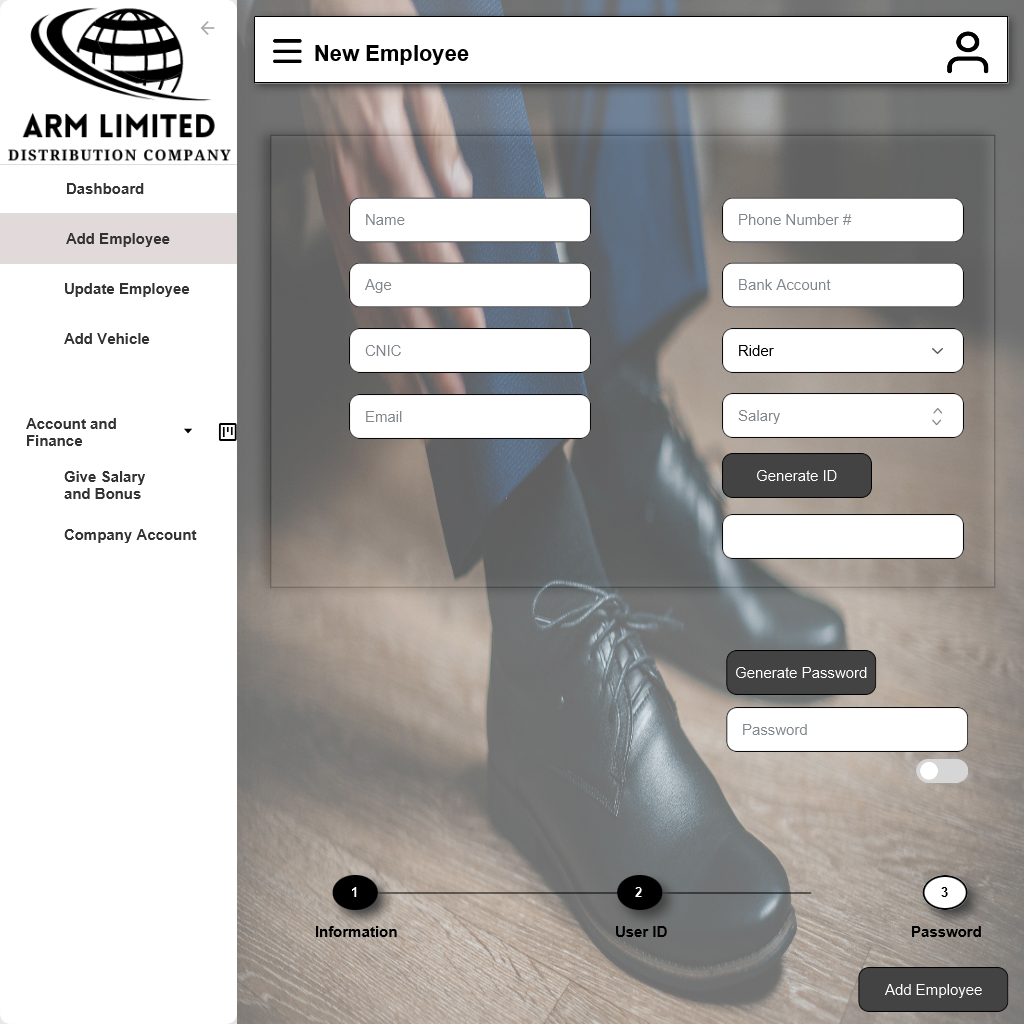
\includegraphics [width=10cm, height=5cm] {first.png} \\ \hline

Validators & 1.	Name: Name should be entered in string.
\newline
2.	Phone Number: It would be of string type with minimum 11 words.
\newline
3.	Age: It would be of int type ranges from 0 to 120.
\newline
4.	Bank Account: It should be input of integers with atleast 15 numbers.
\newline
5.	CNIC: CNIC will be of string type with 13 characters.
\newline
6.	Category: Manager can either select Rider, Supervisor, Sales agent.
\newline
7.	Email: Email will be validated with @gmail.com and it is of string type.
\newline
8.	Salary: It is of int type.
\newline
9.	ID: It is of string type.
\newline
10.	Password: It is of string type.
\newline
. \\ \hline 
\end{tabular}

\end{table}
%%%%%%%%%%%%%%%%%%%%%%%%%%%%%%%%%%%%%%%%%%%%%%%%%%%%%%%%%%%%%%%%%
\begin{table}[H] 
\begin{tabular} {|m{6em}|m{12cm}|}
\hline
Interface ID & I02 \\ \hline
\newline
Name & Update Employee \\ \hline
LinkedUseCase & U06 \\ \hline
UI Screen &\newline 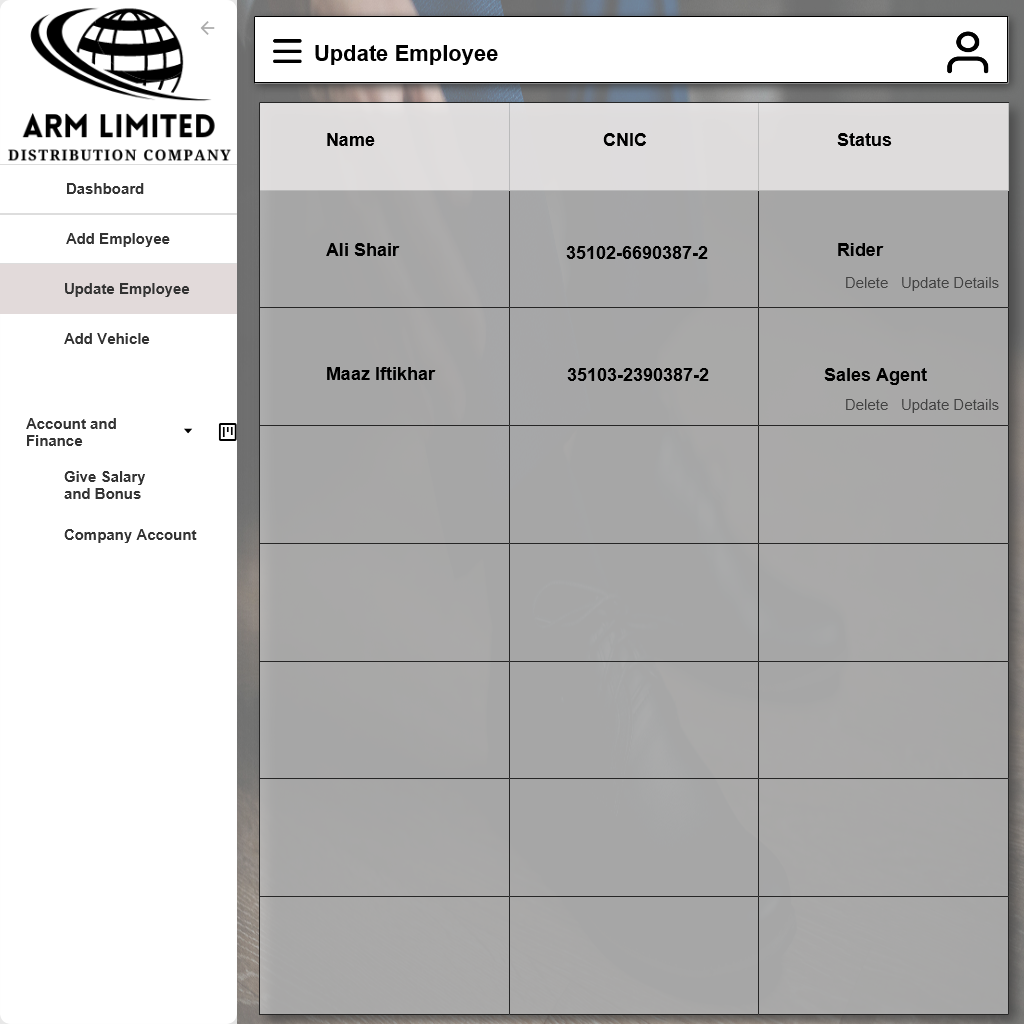
\includegraphics [width=10cm, height=5cm] {2a.png} \\ \hline
\end{tabular}
\end{table}
%%continue table on next page
\begin{table}[H] 
\begin{tabular} {|m{6em}|m{12cm}|}
\hline
     & \newline\newline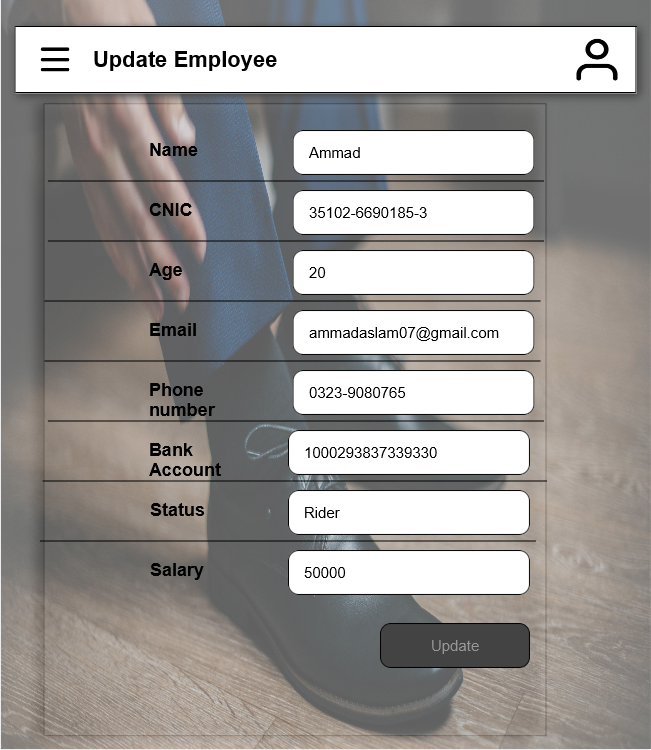
\includegraphics [width=10cm, height=5cm] {3a.png}
     \\ \hline
\newline
Validators &  1.Name: Name should be entered in string.
\newline
2.Phone Number: It would be of string type with minimum 11 words.
\newline
3.Age: It would be of int type ranges from 0 to 120.
\newline
4.Bank Account: It should be input of integers with atleast 15 numbers.
\newline
5.CNIC: CNIC will be of string type with 13 characters.
\newline
6.Category: Manager can either select Rider, Supervisor, Sales agent.
\newline
7.Email: Email will be validated with @gmail.com and it is of string type.
\newline
8.Salary: It is of int type.
\newline
9.ID: It is of string type.
\newline
10.Password: It is of string type.
\newline
\\ \hline
\end{tabular}
\end{table}
%%%%%%%%%%%%%%%%%%%%%%%%%%%%%%%%%%%%%%%%%%%%%%%%%%%%%%%%%
\begin{table}[H] 
\begin{tabular} {|m{6em}|m{12cm}|}
\hline
Interface ID & I03 \\ \hline
\newline
Name & Give Salary and Bonus\\ \hline
LinkedUseCase & U04, U05 \\ \hline
UI Screen &\newline 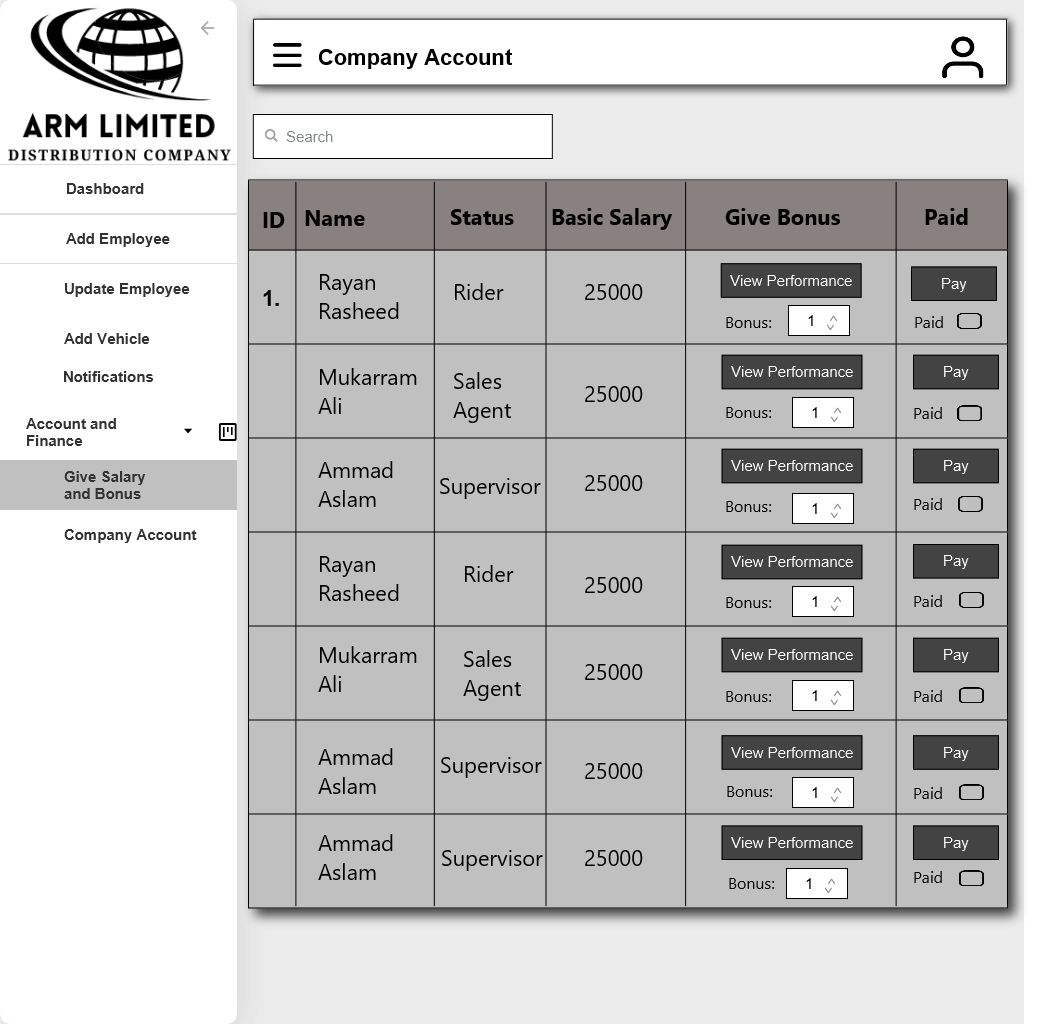
\includegraphics [width=10cm, height=5cm] {r.png} \\ \hline
Validators &  1. Searching: Searching will be according to the name of the employee.
\newline
2. Checkbox: If the salary is paid then it will be checked otherwise it will be unchecked.
\newline
3. Bonus: It should be of int type.
\\ \hline
\end{tabular}
\end{table}
%%%%%%%%%%%%%%%%%%%%%%%%%%%%%%%%%%%%%%%%%%%%%%%%%%%%%%%%%%%%%%%%%5
\begin{table}[H] 
\begin{tabular} {|m{6em}|m{12cm}|}
\hline
Interface ID & I04 \\ \hline
\newline
Name & Company account\\ \hline
LinkedUseCase & U03 \\ \hline
UI Screen &\newline 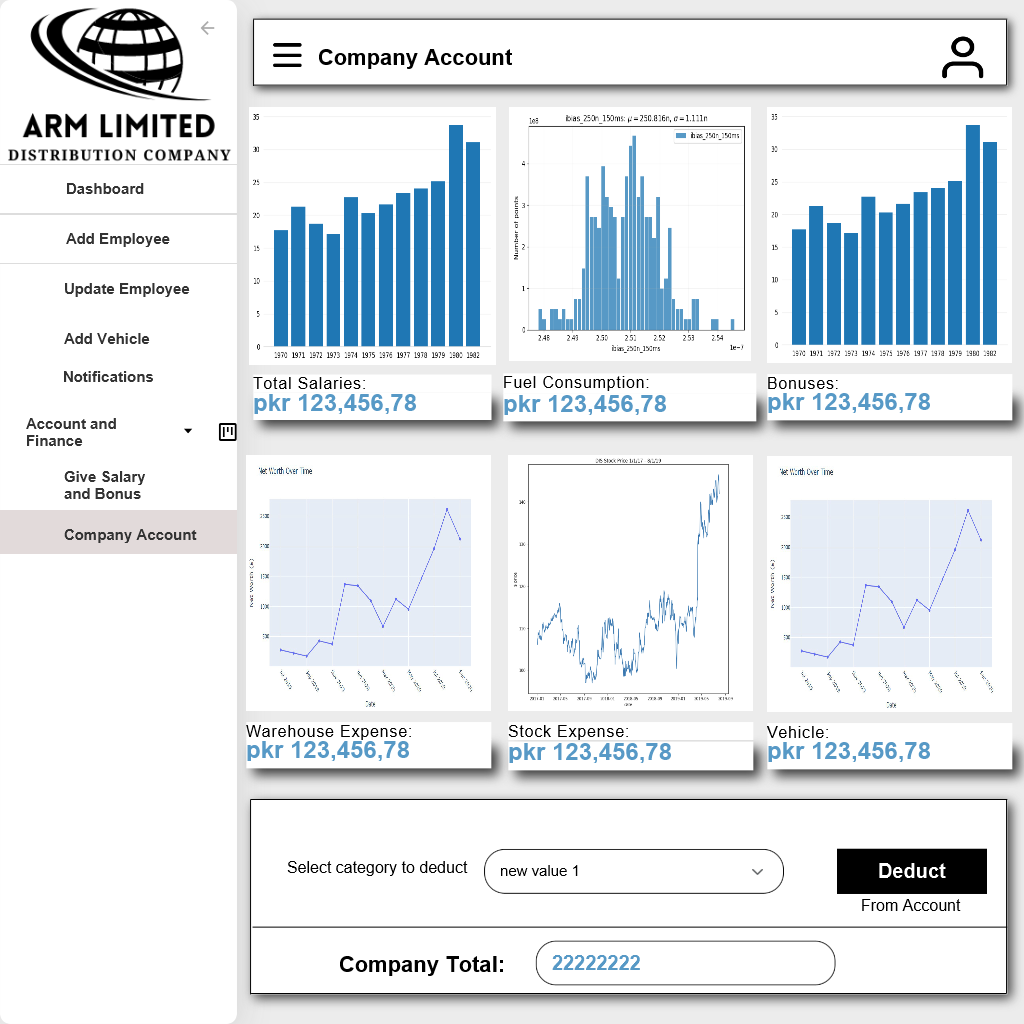
\includegraphics [width=10cm, height=5cm] {4a.png} \\ \hline
Validators &  1. Select Category: It is of dropdown menu that contains the value of string type.
\newline
2. Company Total: It contain the company total in int.
\\ \hline
\end{tabular}
\end{table}
%%%%%%%%%%%%%%%%%%%%%%%%%%%%%%%%%%%%%%%%%%%%%%%%%%%%%%%%%%%%%%%%
\begin{table}[H] 
\begin{tabular} {|m{6em}|m{12cm}|}
\hline
Interface ID & I05 \\ \hline
\newline
Name & Buy Stock\\ \hline
LinkedUseCase & U09 \\ \hline
UI Screen &\newline 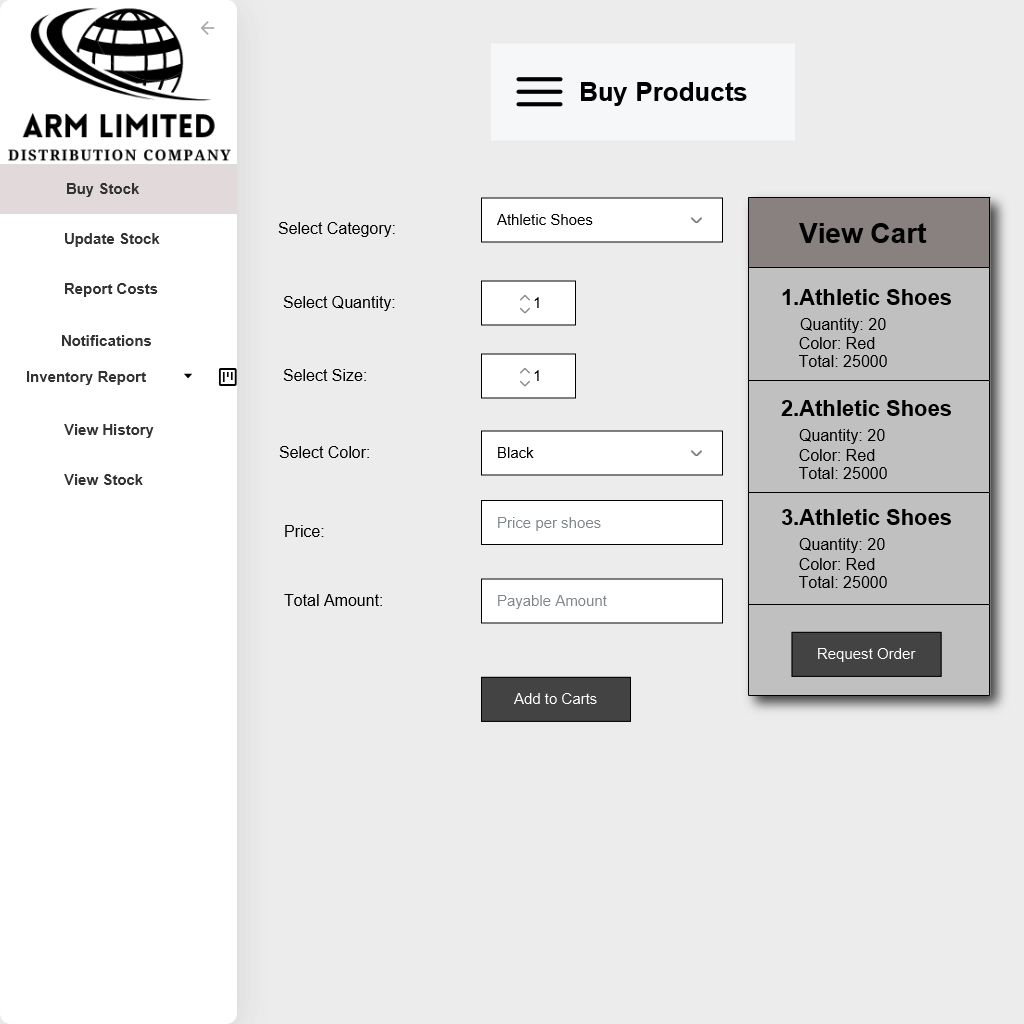
\includegraphics [width=10cm, height=5cm] {5a.png} \\ \hline
Validators &  1. Select Quantity: It is int type.
\newline
2. Select Size: It is int type
3. Price: It is of int type
4. Total Amount: It is of int type
\\ \hline
\end{tabular}
\end{table}
%%%%%%%%%%%%%%%%%%%%%%%%%%%%%%%%%%%%%%%%%%%%%%%%%%%%%5

\begin{table}[H] 
\begin{tabular} {|m{6em}|m{12cm}|}
\hline
Interface ID & I06 \\ \hline
\newline
Name & Update Stock\\ \hline
LinkedUseCase & U10 \\ \hline
UI Screen &\newline 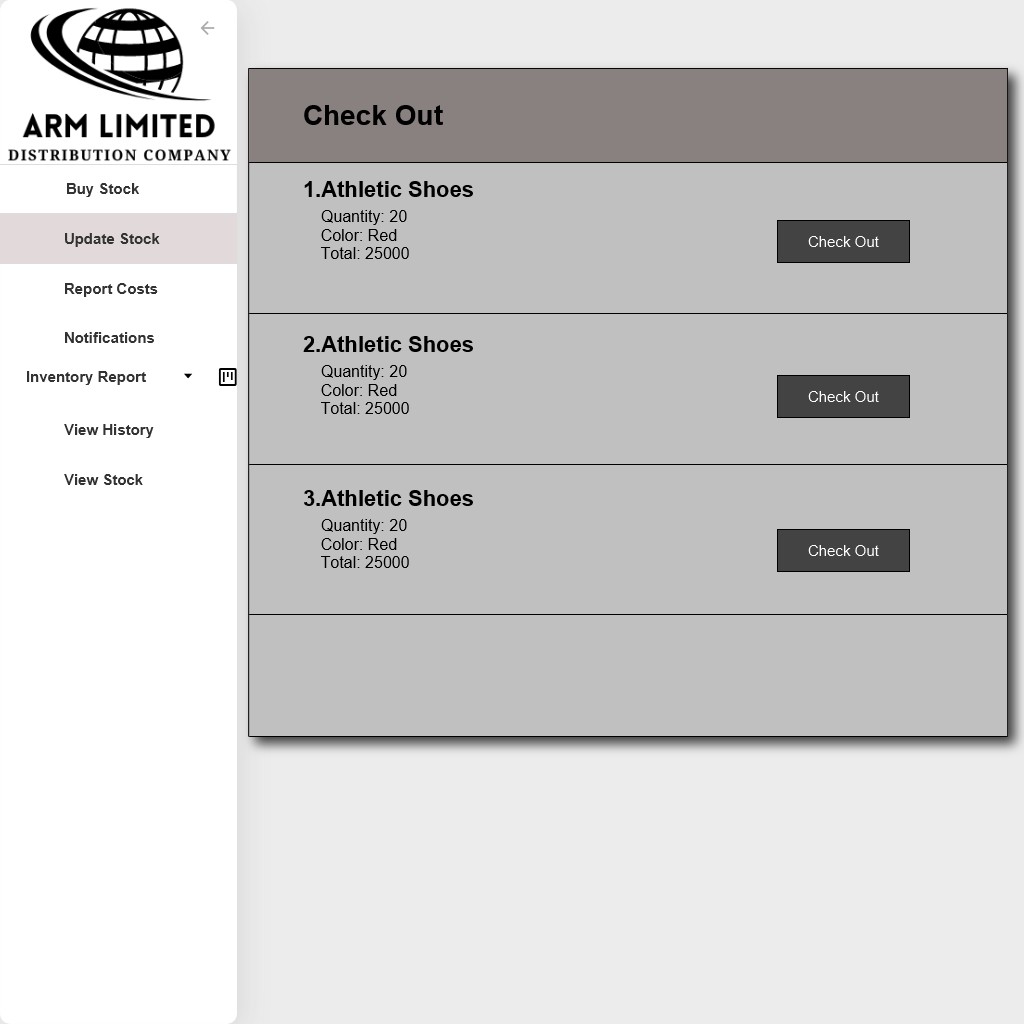
\includegraphics [width=10cm, height=5cm] {6a.png} \\ \hline
Validators &  1. Check out button will be working when the order will be delivered.
\\ \hline
\end{tabular}
\end{table}

%%%%%%%%%%%%%%%%%%%%%%%%%%%%%%%%%%%%%%%%%%%%%%%%%%%%%%%%%%%%%%%%%
\begin{table}[H] 
\begin{tabular} {|m{6em}|m{12cm}|}
\hline
Interface ID & I07 \\ \hline
\newline
Name & View History\\ \hline
LinkedUseCase &  U21 \\ \hline
UI Screen &\newline 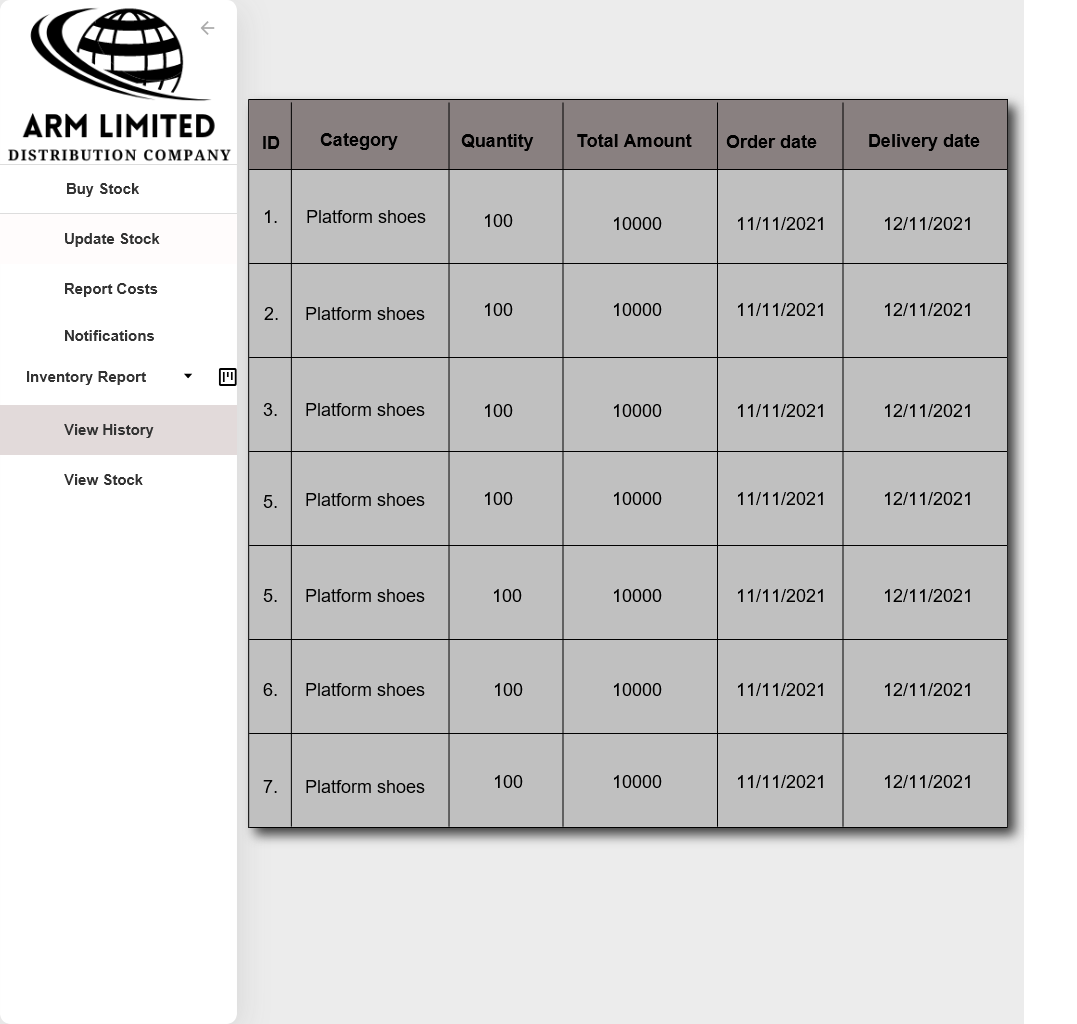
\includegraphics [width=10cm, height=5cm] {8a.png} \\ \hline

\end{tabular}
\end{table}
%%%%%%%%%%%%%%%%%%%%%%%%%%%%%%%%%%%%%%%%%%%%%%%%%%%%%%%%%%%%%%%%%%%%%%%%%%%%%
\begin{table}[H] 
\begin{tabular} {|m{6em}|m{12cm}|}
\hline
Interface ID & I08 \\ \hline
\newline
Name & View Stock\\ \hline
LinkedUseCase & U22  \\ \hline
UI Screen &\newline 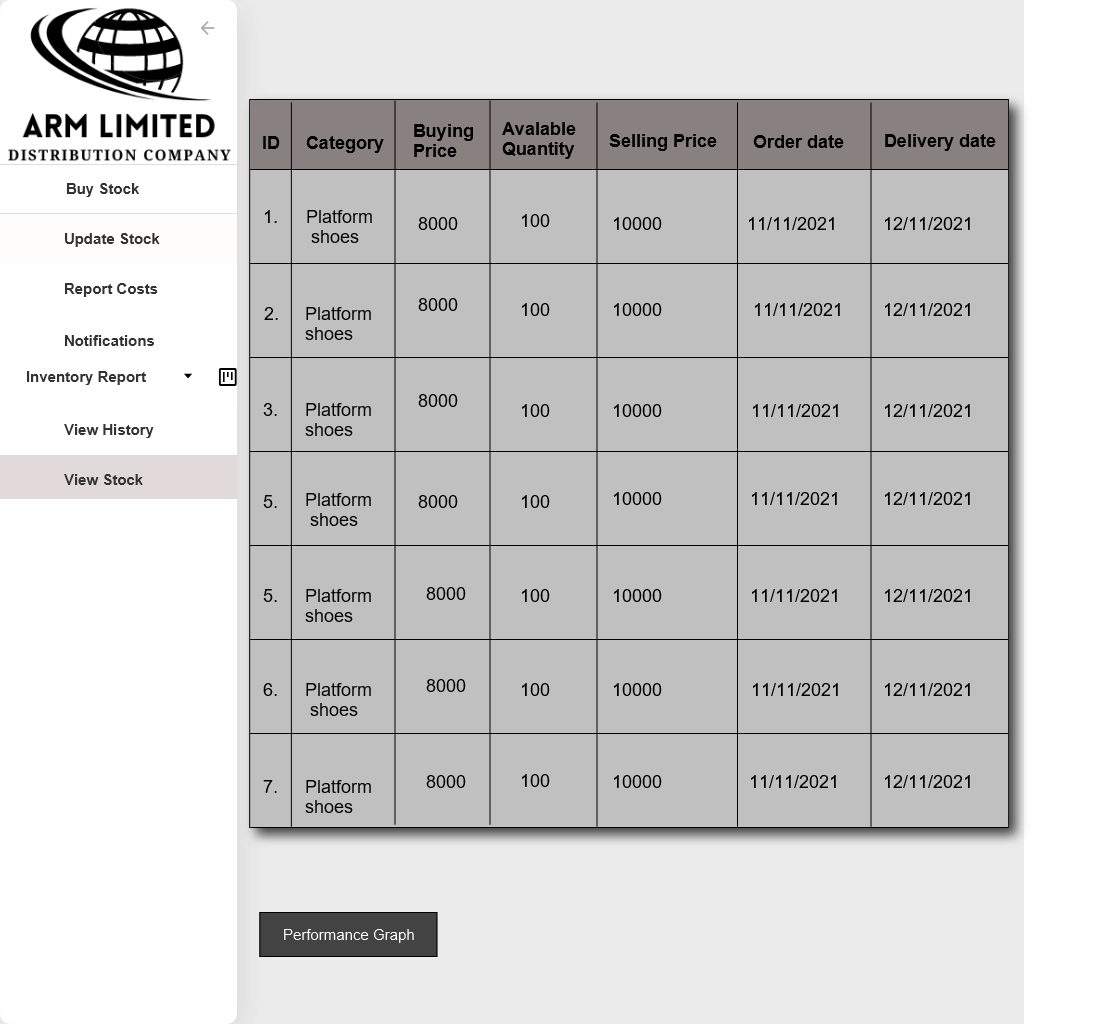
\includegraphics [width=10cm, height=5cm] {9.png} \\ \hline

\end{tabular}
\end{table}
%%%%%%%%%%%%%%%%%%%%%%%%%%%%%%%%%%%%%%%%%%%%%%%%%%%%%%%%%%%%
\begin{table}[H] 
\begin{tabular} {|m{6em}|m{12cm}|}
\hline
Interface ID & I09 \\ \hline
\newline
Name & Report Costs\\ \hline
LinkedUseCase & U12 \\ \hline
UI Screen &\newline 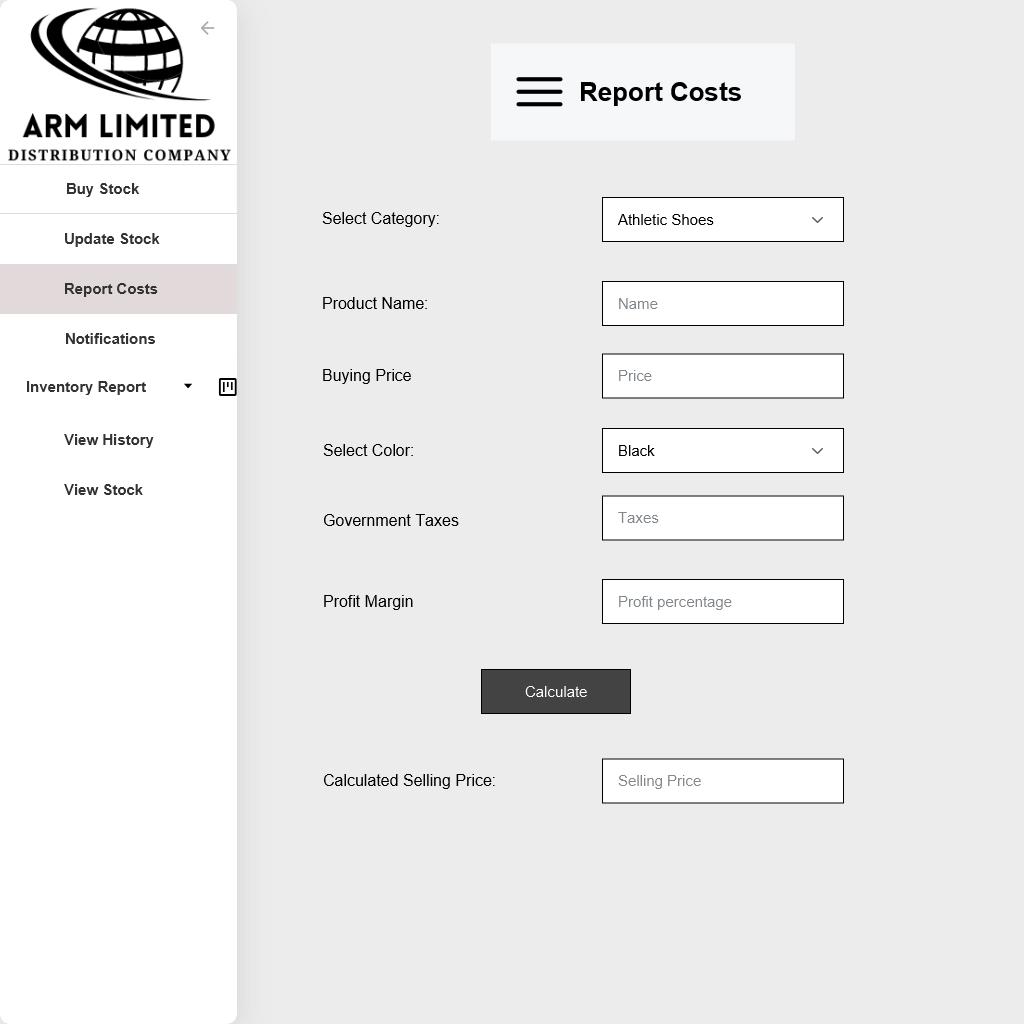
\includegraphics [width=10cm, height=5cm] {7a.png} \\ \hline
Validators &  1. Name is of string type.
\newline
2. Price is of int type
\newline
3. Taxes are of float type.
\newline
4. Profit margin is also of float type.
\newline
5. Selling price is also of float type.
\\ \hline
\end{tabular}
\end{table}
%%%%%%%%%%%%%%%%%%%%%%%%%%%%%%%%%%%%%%%%%%%%%%
\section{Classes}
\begin{table}[H]
\begin{tabular}{|l|l|l|l|l|}
\hline
Class Name          & Software/ Domain & \begin{tabular}[c]{@{}l@{}}Is Abstract \\ (Yes/No)\end{tabular} & \begin{tabular}[c]{@{}l@{}}Is Singleton \\ (Yes/No)\end{tabular} & \begin{tabular}[c]{@{}l@{}}Is the class will have \\ parametrized constructor \\ (Yes/No)\end{tabular} \\ \hline
Manager             &                  & No                                                              & No                                                               & Yes                                                                                                    \\ \hline
SalesAgent          &                  & No                                                              & No                                                               & Yes                                                                                                    \\ \hline
InventorySupervisor &                  & No                                                              & No                                                               & Yes                                                                                                    \\ \hline
Rider               &                  & No                                                              & No                                                               & Yes                                                                                                    \\ \hline
User                &                  & No                                                              & No                                                               & Yes                                                                                                    \\ \hline
Employee            &                  & Yes                                                             & No                                                               & Yes                                                                                                    \\ \hline
UserCrud            &                  & No                                                              & Yes                                                              & No                                                                                                     \\ \hline
Client              &                  & No                                                              & No                                                               & Yes                                                                                                    \\ \hline
Account             &                  & No                                                              & No                                                               & Yes                                                                                                    \\ \hline


\end{tabular}
\end{table}

\begin{table}[H]
\begin{tabular}{|l|l|l|l|l|}
\hline
Class Name       & Software/ Domain & \begin{tabular}[c]{@{}l@{}}Is Abstract \\ (Yes/No)\end{tabular} & \begin{tabular}[c]{@{}l@{}}Is Singleton\\  (Yes/No)\end{tabular} & \begin{tabular}[c]{@{}l@{}}Is the class will have \\ parametrized constructor \\ (Yes/No)\end{tabular} \\ \hline
Path             &                  & No                                                              & No                                                               & Yes                                                                                                    \\ \hline
Attendance       &                  & No                                                              & No                                                               & Yes                                                                                                    \\ \hline
AttendanceRecord &                  & No                                                              & Yes                                                              & No                                                                                                     \\ \hline
Product          &                  & No                                                              & No                                                               & Yes                                                                                                    \\ \hline
Item             &                  & No                                                              & No                                                               & Yes                                                                                                    \\ \hline
Order            &                  & No                                                              & No                                                               & Yes                                                                                                    \\ \hline
OrderLine        &                  & No                                                              & Yes                                                              & No                                                                                                     \\ \hline
ProductCRUD      &                  & No                                                              & Yes                                                              & No                                                                                                     \\ \hline
Bill             &                  & No                                                              & No                                                               & Yes                                                                                                    \\ \hline
\end{tabular}
\end{table}

\section{Object Oriented Features}
\subsection{Composition:}

\begin{center}
	 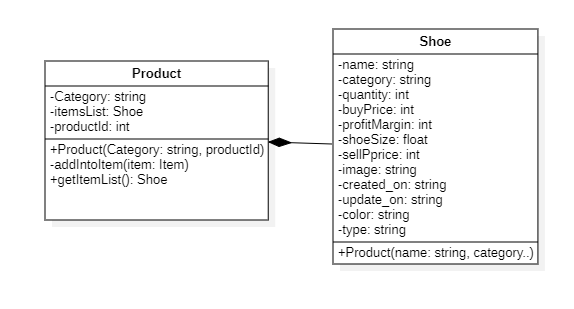
\includegraphics[width=170mm,height=120mm]{1.png}
  \captionof{figure}{Example 1: Composition between Product and shoe.}
\end{center}

\begin{center}
	 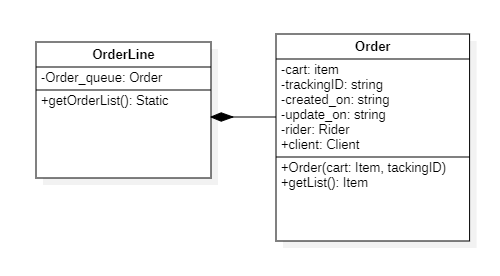
\includegraphics[width=170mm,height=70mm]{2.png}
      \captionof{figure}{Example 2: Composition between Product and shoe.}
\end{center}

\subsection{Inheritance:}
\begin{center}
	 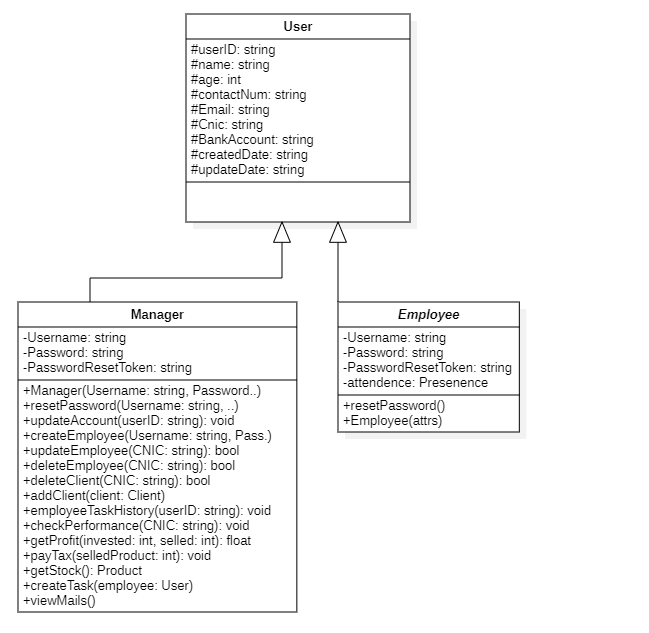
\includegraphics[width=199mm,height=115mm]{3.png}
      \captionof{figure}{Example 1: Extending the User class from Manager and Employee.}
\end{center}
\begin{center}
	 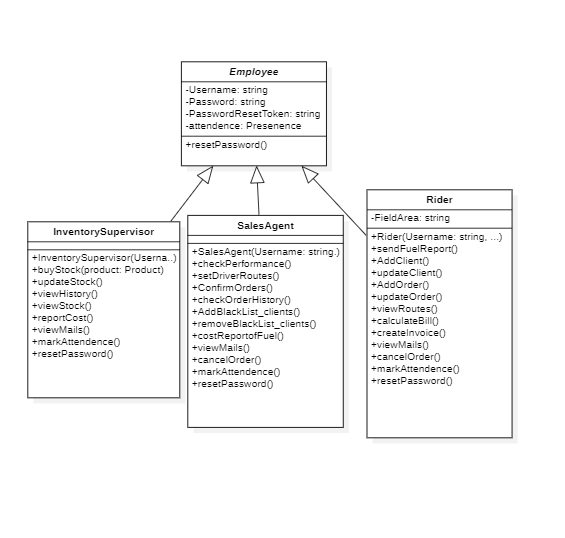
\includegraphics[width=199mm,height=170mm]{4.png}
      \captionof{figure}{Example 2: Extending the employee from inventory supervisor, driver and sales agent.}
\end{center}

\subsection{Multi-Level Inheritance:}
\begin{center}
	 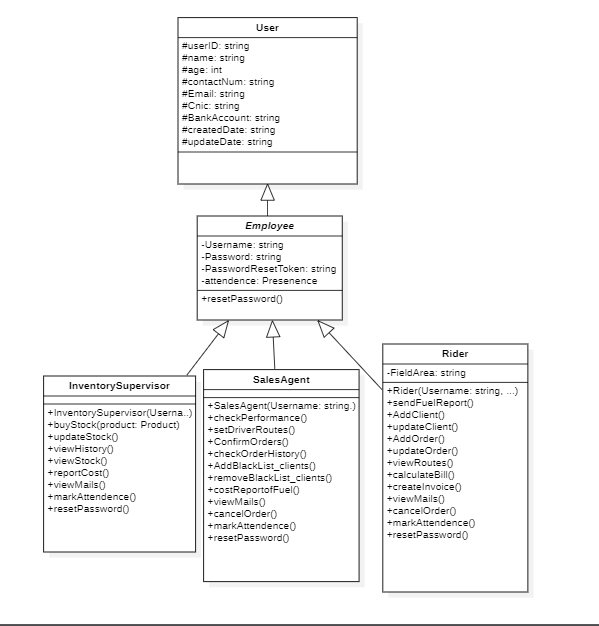
\includegraphics[width=199mm,height=180mm]{5.png}
      \captionof{figure}{Example: Extending the User class from Employee and Employee from Inventory Supervisor, Sales Agent, and Rider class.}
\end{center}

\subsection{Multiple Inheritance:}
\begin{center}
	 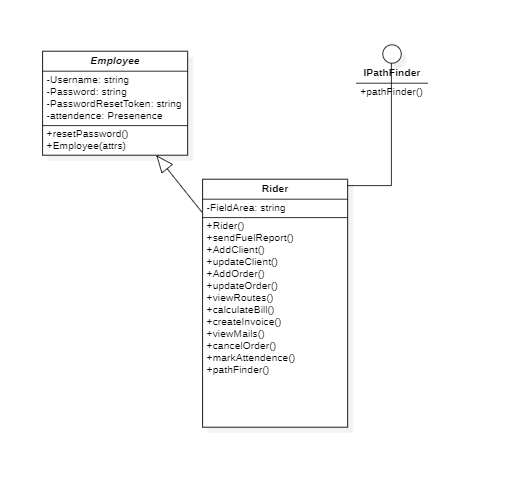
\includegraphics[width=199mm,height=180mm]{6.png}
      \captionof{figure}{Example: Employee and I Pathfinder are extended the Rider class.}
\end{center}

\subsection{Polymorphism:}
\begin{center}
	 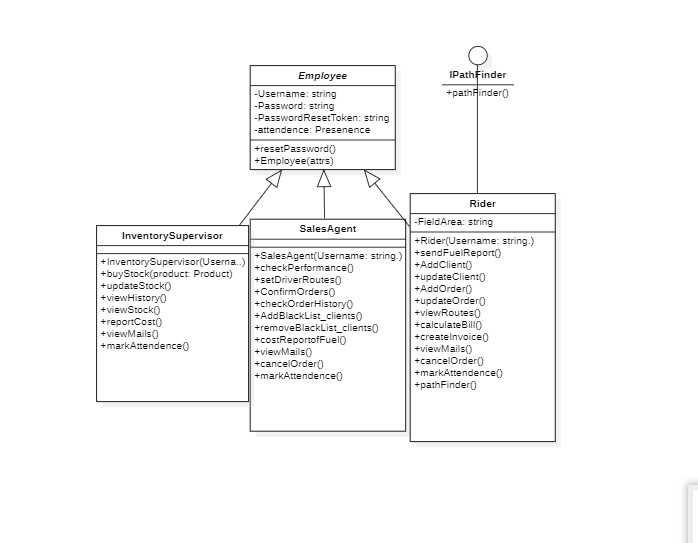
\includegraphics[width=199mm,height=200mm]{7.png}
      \captionof{figure}{Example: Inventory Supervisor, Rider, and Sales Agent share common properties using abstract function in super class and defining it in sub-classes.}
\end{center}

\section{Detailed Object-Oriented Design:}
\begin{center}
	 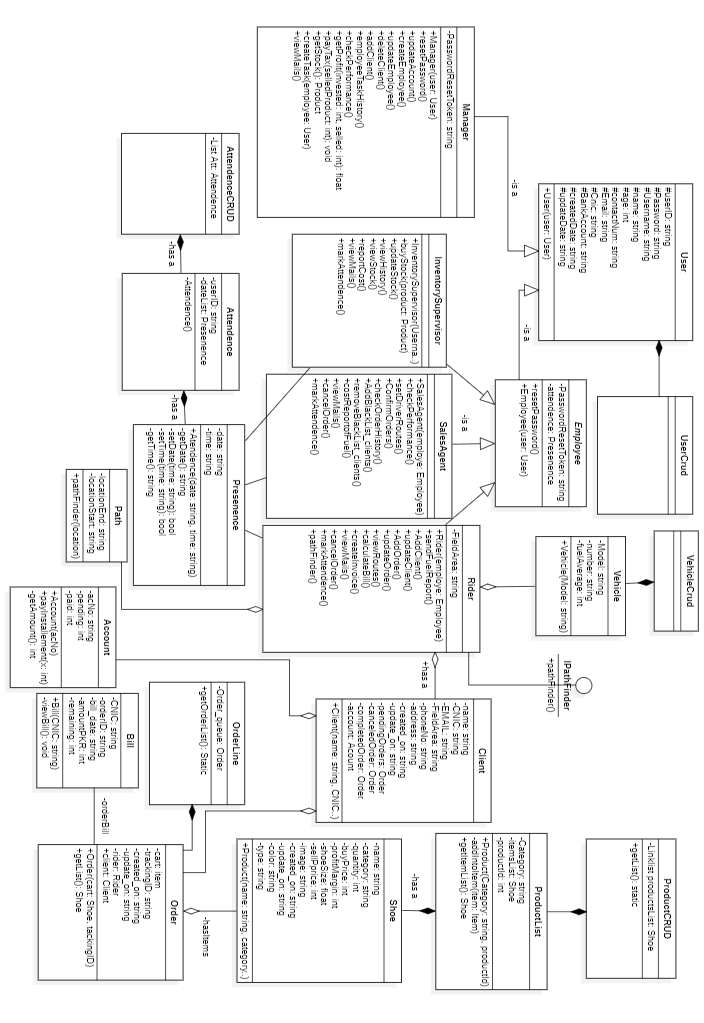
\includegraphics[width=170mm,height=210mm]{8.png}
      }
\end{center}


\end{document}
